\section{Combustion Instabilities}

\subsection{Primary and Secondary Thermoacoustic Instabilities}

Combustion for engineering applications typically happens in systems of chambers, connected by long ducts. Although the chemical and hydrodynamic scales remain relatively short, and are localised to specific areas, e.g. the combustion chamber, acoustics travel throughout the system without significant damping due to the acoustically reflective materials used. Hence, the dominant acoustic eigenmodes of a system are therefore free to interact with the flame as they please. The resulting \emph{thermoacoustic} (TA) instabilities are classed as a form of chamber instability due to the reliance of the flame's spontaneous acoustics on specific geometries. The effect of thermoacoustics was first noticed in \cite{mallard1883RecherchesExperimentalesTheoriques}, where it was observed that flames can produce their own acoustic oscillations. Following this, \cite{rayleigh1896TheorySound} introduced a theoretical condition for a \emph{primary} TA instability, so called the \emph{Rayleigh criterion}, where fluctuations in pressure and heat release from the flame are amplified whenever they are in phase. To explain this in more detail, periodic changes to pressure are coupled to changes in acoustic velocity. This has a convective effect on the shape of the curved, hydrodynamically unstable \cite{darrieus1945PropagationFrontFlamme,landau1944TheorySlowCombustion,matalon2018DarrieusLandauInstability} flames, resulting in an oscillation of the total heat release. This causes further oscillations to the radiated acoustic pressure from the flame, which closes this feedback mechanism. The primary TA instability can, hence, only occur when the oscillating pressure around the flames results in heat release oscillations which add to the acoustic pressure amplitude. Mathematically, instability is triggered whenever:
\begin{equation}
\rm{RI} \equiv \oint p' Q' \dd{t} > 0
\end{equation}
where $\rm{RI}$ is the \emph{Rayleigh Index}, $p'$ and $Q'$ represent fluctuations in the pressure and total heat release, respectively. The closed integral sign represents the integral over a single of the above mentioned periods. This statement translates to the statement that $p'$ and $Q'$ must be in phase with one another for instability to occur. This phase is controlled by the acoustics of the combustion chamber itself so small changes to combustor system's geometry can result in large qualitative changes to stability. When they are in phase, the feedback loop takes the form of a clockwise p-V cycle \cite{polifke2004CombustionInstabilities}, equivalent to an Otto cycle. This means the mechanism can generate mechanical work which, when confined to an engine, can take the form of a damaging force on engine parts, such as the damage observed in \cite{lieuwen2006CombustionInstabilitiesGas}.

Stroboscopic imagery of flames propagating through tubes are shown in \cite{guenoche1964ChapterFlamePropagation} and made by periodically exposing the same film to the flame's light using a rotating drum. By establishing four different test configurations of these ducted flames (each of the two ends being either closed or open to the environment), the experiments establish flame structures common between these test cases. For one, all test cases have a flame which decelerates after ignition. They also observe oscillations in the flame's shape, not yet explained by the primary instability mechanism. These flame oscillations, \cite{guenoche1964ChapterFlamePropagation} concludes, are the result of the interaction of the acoustic oscillation of the gas, determined by the tube's acoustics, and the flame front.

\begin{figure}[t]
\centering
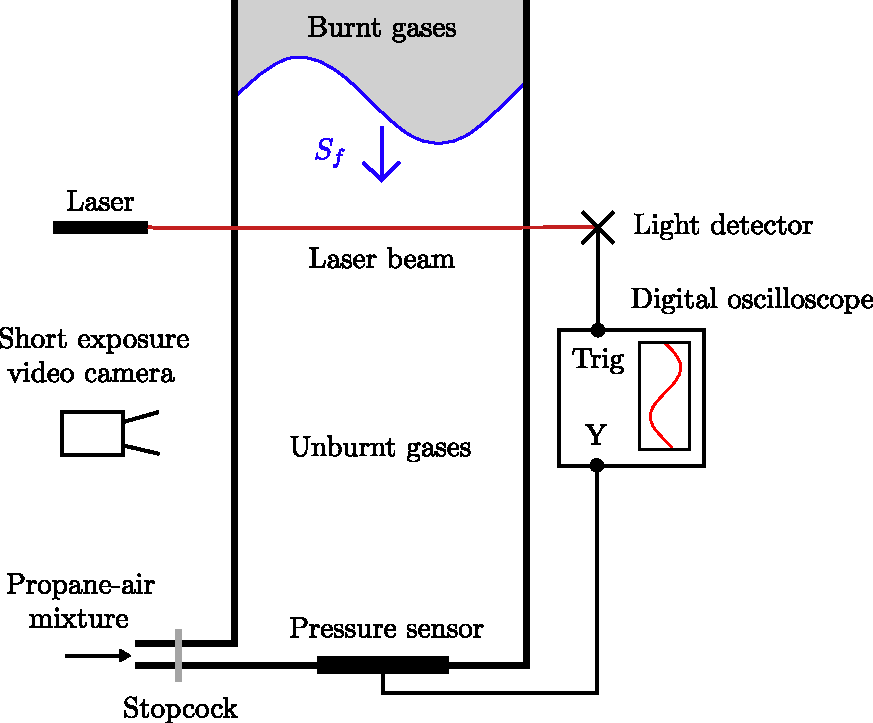
\includegraphics[scale=0.6]{assets/imgs/Searby-92.pdf}
\caption{Illustration of the experimental apparatus of \cite{searby1992AcousticInstabilityPremixed}.}
\label{fig:searby-experiment}
\end{figure}

An insightful experiment into thermoacoustics was performed later in 1992 by Searby \cite{searby1992AcousticInstabilityPremixed} and studied relationships between a cylindrical tube's acoustics as well as the speed and shape of the premixed flame within. The experimental apparatus is depicted in \fig{fig:searby-experiment}. Propane-air mixtures were lit at the top end of the tube and propagate down, with any acoustic disturbance detected by a pressure sensor at the bottom. Additionally, a small laser beam was place near the top of the tube to detect the flame as thermal gradients deflect the light. This triggers a digital oscilloscope to record pressure disturbances from the pressure sensor. A short exposure video camera was used to image the flame surface and observe its structure as it propagates. Since propane (C$_3$H$_8$) is a relatively heavy fuel with a species diffusion rate lower than methane's, the lean and stoichiometric mixtures used have Lewis numbers which are never below the critical Lewis number, $\Le_\rm{crit}$, required for \emph{thermodiffusive instabilities} \cite{zeldovich1944TheoryCombustionDetonation,barenblatt1962DiffusionalThermalStabilIty,sivashinsky1977DiffusionalThermalTheoryCellular} to have an effect. Note that the downward propagating flames will have been somewhat stabilised by the \emph{Rayleigh-Taylor} (RT) instability. The primary instability is observed alongside a secondary, which is associated with a different feedback mechanism, acoustic envelopes and flame dynamics.

\begin{figure}[t]
\centering
\begin{subfigure}{0.49\textwidth}
\centering
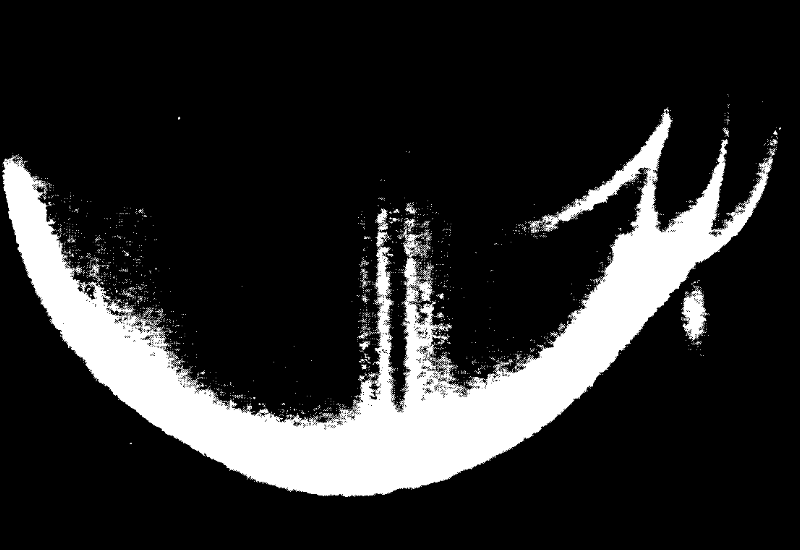
\includegraphics[height=5cm]{assets/imgs/Searby-92-flame_a.png}
\caption{}
\label{fig:Searby-92_flames_a}
\end{subfigure}
\hfill
\begin{subfigure}{0.49\textwidth}
\centering
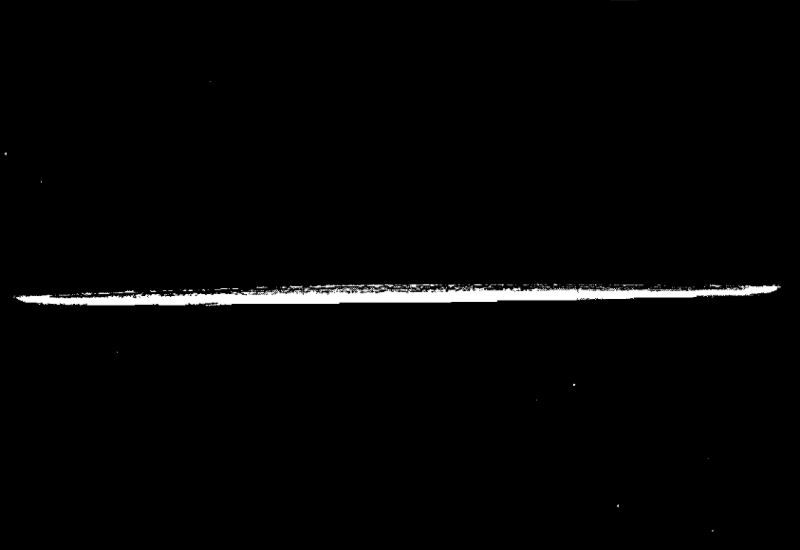
\includegraphics[height=5cm]{assets/imgs/Searby-92-flame_b.png}
\caption{}
\label{fig:Searby-92_flames_b}
\end{subfigure}

\vspace*{3mm}

\begin{subfigure}{0.49\textwidth}
\centering
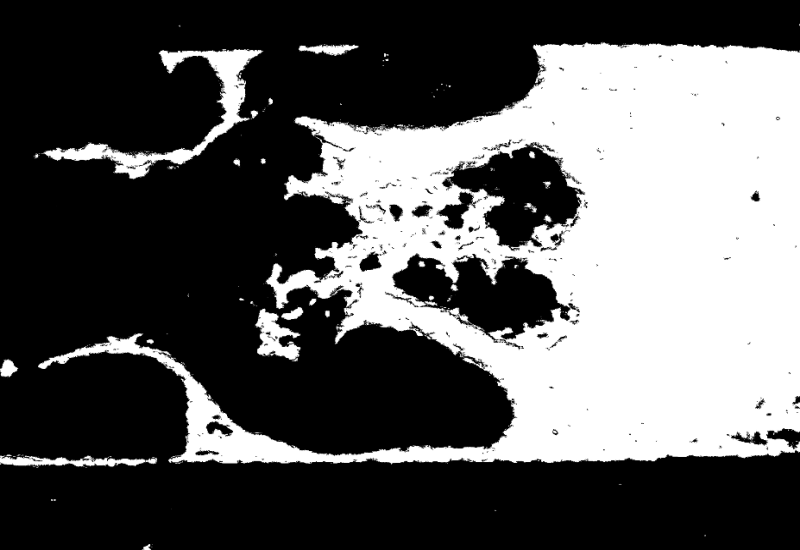
\includegraphics[height=5cm]{assets/imgs/Searby-92-flame_c.png}
\caption{}
\label{fig:Searby-92_flames_c}
\end{subfigure}
\hfill
\begin{subfigure}{0.49\textwidth}
\centering
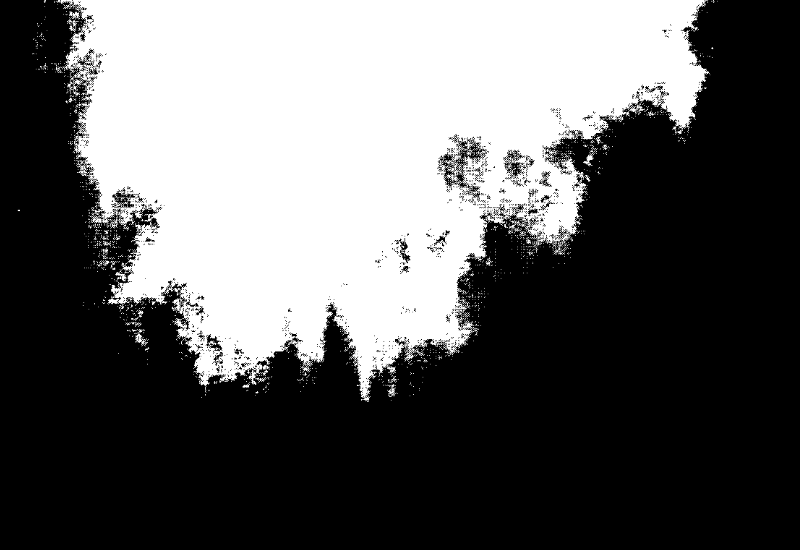
\includegraphics[height=5cm]{assets/imgs/Searby-92-flame_d.png}
\caption{}
\label{fig:Searby-92_flames_d}
\end{subfigure}
\caption{Photos, courtesy of \cite{searby1992AcousticInstabilityPremixed}, of flames at different stages of TA response. (a) shows the characteristic curved shape of a hydrodynamically unstable flame before any acoustics are significantly effecting the flame shape. (b) is a flame flame under the effect of the primary TA instability. (c) shows a cross-sectional slice of a flame rotated by $90\degree$ under the secondary instability. (d) shows a flame after the breakdown of cellular structures, which leads to a self-turbulent flame.}
\label{fig:Searby-92_flames}
\end{figure}

Initially, the flame curves as a result of the hydrodynamic instability, as photographed in \fig{fig:Searby-92_flames_a}. After some time, the acoustic amplitude increases due to primary instability. As the acoustic amplitude increases the flame flattens, seen in \fig{fig:Searby-92_flames_b}, resulting in a decrease in flame speed due to the decreased fuel consumption rate. In some of the flames tested, only the primary instability is observed, but in some others it progresses beyond this to the secondary instability -- often before the fully flattened flame is observed. At the immediate onset of the secondary instability, if it occurs, a cellular structure of a given wavenumber appears and corresponds to a rapid increase in the acoustic amplitude. This onset is much more rapid than for the primary instability, and eventually the cellular structure transitions into a symmetric flame structure similar to \fig{fig:Searby-92_flames_c}. Provided the flame has not yet reached the end of the tube it may also devolve into a self-turbulent flame similar to that shown in \fig{fig:Searby-92_flames_d}. The flame structures resulting from the secondary instability have significantly higher velocities as a result of their massively increased flame surface area and are viewed as a violent instability. The self-turbulent regime marks a significant decline to the acoustic amplitude as there is no regular release of pressure fluctuations from the flame.
% Flat flame under primary can be seen as a limit cycle

The secondary instability mechanism is seen by Searby \cite{searby1992AcousticInstabilityPremixed} as a \emph{parametric instability}. Searby and Rochwerger \cite{searby1991ParametricAcousticInstability} pose this system as a Mathieu equation by incorporating the effect of acoustic force into an equation for flame position under the influence of gravity, which is otherwise written as a damped harmonic oscillator \cite{searby1986WeaklyTurbulentWrinkled}. The Mathieu equation demonstrates a canonical example of parametric instability, since solutions remain unbounded whenever the forcing acoustic frequency is double that of the natural frequency implied by the flame in its damped harmonic oscillation. Physically this corresponds to a flame with a structure that oscillates with a period double that of the acoustic period.

% EXPLAIN WHAT S_L AND L_TH ARE
\begin{figure}[t]
\centering
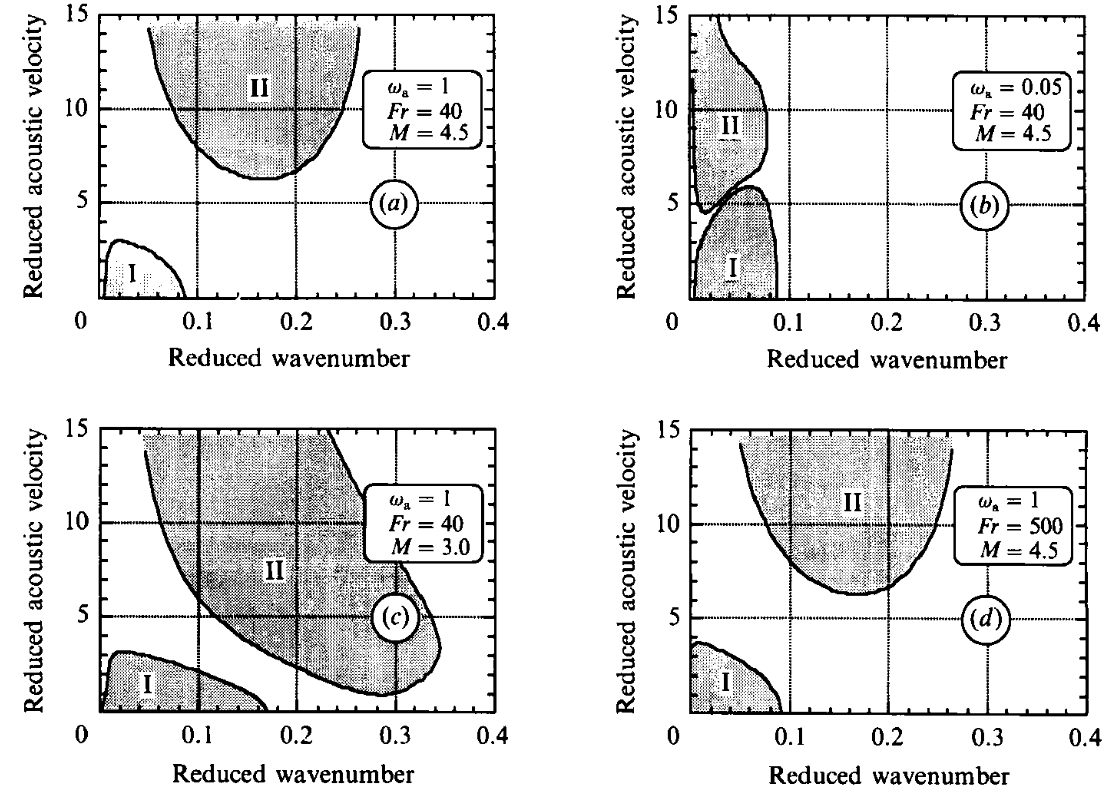
\includegraphics[height=11cm]{assets/graphs/thermoacoustic-stability.png}
\caption{Stability diagrams, courtesy of \cite{searby1991ParametricAcousticInstability}, for four different values of $ω_a$, $\Fr$ and $\Mk$. The regions I and II are regions of instability for the plane flame. Reduced wavenumbers are given as $k l_\rm{th}$ and reduced acoustic velocities are $u_a / S_L$.}
\label{fig:ta-stab}
\end{figure}

Using this formation of the flame front as solutions to the Mathieu equation, \cite{searby1991ParametricAcousticInstability} calculates regions of flame instability for a planar flame as functions of perturbation wavenumber $k$, acoustic velocity $u_a$ (the amplitude of which can be thought of as the intensity or volume of sound), acoustic frequency $ω_a$, Froude number $\Fr$ (representing non-dimensional inverse of gravitational forcing) and Markstein number $\Mk$ (a crucial flame parameter connecting the sensitivity of the flame's speed to perturbations to its surrounding hydrodynamics). They then plot these regions in \fig{fig:ta-stab}. Note that these plots do not acoustic instability mentioned above, but their effect on flame stability for a planar flame. In all the plots, there are two disjoint regions of flame instability. The region I represents hydrodynamic instability and occurs, as expected, at zero acoustic velocity for some wavenumber interval. This region ends at some finite $u_a$ as the primary acoustic instability eventually overcomes the hydrodynamic one. At non-zero acoustic velocity, region II of flame instability begins, corresponding to the aforementioned parametric instability. Interestingly, some of the graphs show acoustic velocities where regions I and II can coexist for different wavenumber intervals. In these cases, the primary thermoacoustic instability is expected to lead immediately into the secondary instability with no planar flame observed. On the other hand, for those acoustic velocities where neither region is present the planar flame is stable, so we see structures like \fig{fig:Searby-92_flames_b} where the flame has spontaneously flattened before any secondary instability can occur. We also notice that there is a wavenumber in region II which corresponds to the lowest unstable acoustic velocity. This means that once this acoustic velocity is met, only that wavenumber (and wavenumbers close to it) will be present as wrinkles in the flame. Finally, we note that the effect of increased gravity (decreased $\Fr$) on these downward propagating flames has stabilised the very low wavenumbers next to region I as the RT effect actually stabilises the plane flame.

An experiment was also performed by \cite{searby1991ParametricAcousticInstability} to demonstrate these results. A similar apparatus to \fig{fig:searby-experiment} was used, with significant changes being the usage of a loudspeaker in the bottom of the combustion tube to play sounds of wavelength one-quarter or three-quarters of the wavelength of the tube. A porous plate was placed above the loud speaker to remove any turbulence such that our laminar theories can be applied. Using the loud speaker to excite the flame at known volumes and frequencies (which correspond to controlling $u_a$ and $ω_a$, respectively), they observe both the planar and wrinkled flames described above. The sound intensity corresponding to the quietest parametrically unstable flame may then be plotted for a variety of acoustic frequencies, resulting in a curve predicted by the Mathieu equation model described above for a specific Markstein number. This enables the direct estimation of the Markstein number, which remains a difficult challenge and so remains a prevalent technique \cite{delfin2024ThermoacousticParametricInstability}.

Beyond this, TA oscillations have been observed in a variety of experimentation. Methane-air combustion in a cylindrical tube was investigated experimentally in \cite{fichera2001ExperimentalAnalysisThermoacoustic} with data recorded from an optical sensor to detect changes to heat release, a pressure transducer for internal pressure recordings and a microphone for external pressure recordings. TA oscillations were observed and a non-linear analysis into the dynamical behaviour of the flame recordings demonstrate a chaotic nature to these thermoacoustics. The global stability of the flame, which is guaranteed by diffusive effects, is corroborated via calculation of the set of Lyapunov exponents. The thesis \cite{ebieto2017DynamicsPremixedFlames}, provides a detailed setup to gather high-speed imagery, chemiluminescent and pressure data in a variety of TA flames. The effects of a variety of phenomena affecting acoustic stability, such as RT instability, are outlined. Further experimentation is done on premixed flame oscillations in \cite{delfin2024VideoTransientParametric,martinez-ruiz2018VideoPremixedflameOscillations,delfin2024ThermoacousticParametricInstability} and provide high-fidelity imagery of flames under the effects of primary and secondary instability in \cite{delfin2024VideoTransientParametric,martinez-ruiz2018VideoPremixedflameOscillations}.





\subsection{Thermoacoustic Instability Modelling}

\begin{figure}[t]
\centering
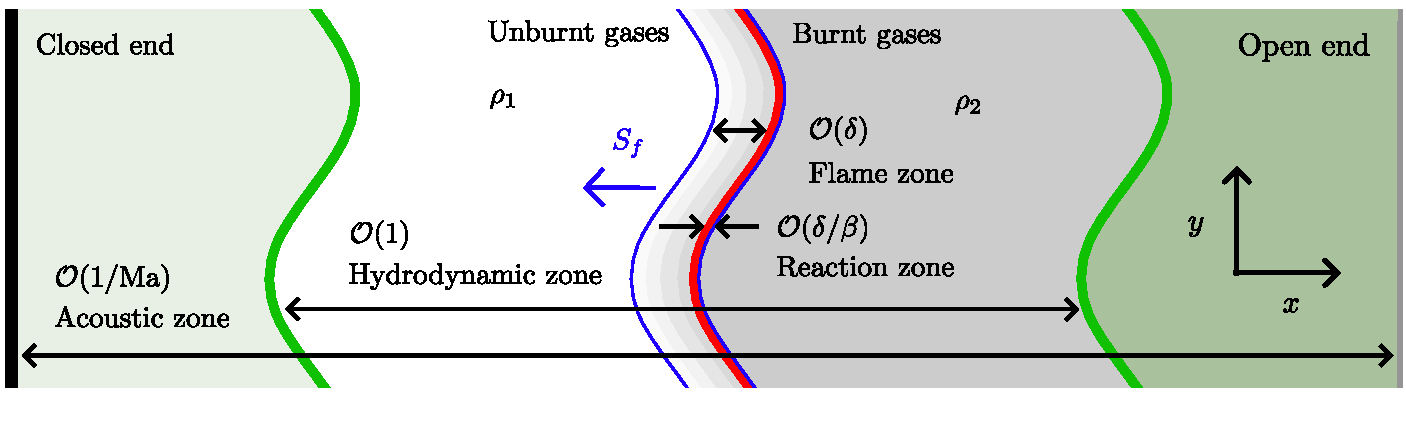
\includegraphics[scale=0.6]{assets/imgs/AW-flame.pdf}
\caption{Diagram showing the model geometry of the multiscale analysis performed by \cite{assier2014LinearWeaklyNonlinear}. The different non-dimensionalised asymptotic scales involved in the full analysis are labeled above the domain.}
\label{fig:AW-flame}
\end{figure}

Later on, work by Assier and Wu \cite{assier2014LinearWeaklyNonlinear} studied the stability of a \emph{flame-flow-acoustic} system, where a freely propagating flame in a closed-open, periodic duct is considered. \fig{fig:AW-flame} illustrates this geometry and is reminiscent of the experimental domain shown in \fig{fig:searby-experiment} of \cite{searby1992AcousticInstabilityPremixed}, excluding any wall boundary layer effects. Results from hydrodynamic flame theory \cite{matalon1982FlamesGasdynamicDiscontinuities,clavin1982EffectsMolecularDiffusion} are used to separate the dynamics within the flame from the outer fluid. This outer region is then separated into the usual $\cl{O}(1)$ hydrodynamic zone and a far-away $\cl{O}(1/\Ma)$ acoustic zone. Further asymptotic analysis is performed in the flame reference frame, coupling the two regions through dynamic jump conditions. A weak non-linearity assumption is made to simplify the flame equation such that linear stability analysis may be performed about the steady solutions to the Michelson-Sivashinsky equation \cite{sivashinsky1977NonlinearAnalysisHydrodynamic,michelson1977NonlinearAnalysisHydrodynamic,matalon2018DarrieusLandauInstability}.

They find that, when the acoustic interaction is included, these solutions are no longer linearly stable and the maximum growth rate of this instability increases significantly with heat release $q$. Non-linear stability analysis is also performed using a solver for the flame position coupled to the dynamical acoustic jump conditions. This is compared to the results of \cite{searby1992AcousticInstabilityPremixed} and they find they are able to qualitatively reproduce the primary instability and the onset of the secondary instability provided the flame parameter is allowed to deviate from its predicted value. In the latter case, the unsteady nature of the acoustic coupling to the flame induces an unsteady RT effect as the acoustic acceleration oscillates into and away from the less dense products. This is viewed as the driving mechanism behind this parametric instability. In a later conference paper, \cite{assier2014CombustionInstabilityModel}, tangential velocity terms are reintroduced and the parameter resulting in the same flame and acoustic behaviour as seen in \cite{searby1992AcousticInstabilityPremixed} more closely match the expected value. These results are surprisingly fruitful given they assume weak non-linearity in the face of the large heat releases the model is tested against.

In \cite{jun2023ParametricInstabilityPropagating} the secondary instability in hydrogen enriched methane-air flames is studied numerically in an open-ended tube. The structure of their flames under the full non-linear effect of the secondary instability is an impressive match to the experiment of \cite{ebieto2017DynamicsPremixedFlames}, in spite of a lack of convergence in the phase of sub-harmonic oscillations to the flame front (between grid spacings of 100 $μ$m to 50 $μ$m). They also find that the Rayleigh Index, $\rm{RI}$ is a good indicator for the onset of the secondary instability and that the violent acoustic output of this parametric instability may also be attributed to the changes in flame surface area strengthening oscillations in heat release which cause the thermoacoustic effect. They determine the main reason secondary instability is not seen in simulations of faster flames is simply that the tube is not long enough for the instability to develop before the flames reach the end of the tube. This validates a desire to model the behaviour of flames which are held in place, such as those in a held in place by combustor geometry in counterflow.


% veiga-lopez2020ThermoacousticAnalysisLean
% - Experimental study of H2-air flames in Hele-Shaw cells
% - Study effects of confinement due to cell geometry, gravity and mixture composition on thermoacoustic oscillations
% - Heat loss effects are most prevalent for very thin cells, where ...




\subsection{G-Equation Model}

% Aimee morgans




\subsection{Low-Order Thermoacoustic Modelling}

% n-tau models
% control theory stuff i don't understand

\cite{juniper2018SensitivityNonlinearityThermoacoustic}




\subsection{Instability Control}

\begin{figure}[t]
\centering
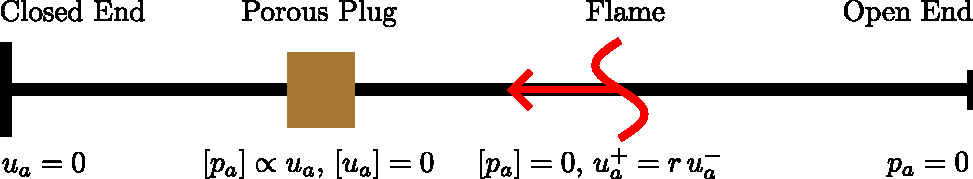
\includegraphics[scale=0.6]{assets/imgs/GP-model.pdf}
\caption{Illustration of the one-dimensional model considered by \cite{gaton-perez2025MitigationThermoacousticInstabilities}, where boundary conditions for each component of the model are shown.}
\label{fig:GP-model}
\end{figure}

Simpler analysis is performed by Gatón-Pérez et al. \cite{gaton-perez2025MitigationThermoacousticInstabilities} to evaluate the eigenstates of a one-dimensional closed-open tube containing a porous plug and a flame. Using Darcy's law to model the plug and assuming linear acoustics, the acoustic eigenmodes of the tube are found numerically. Experimental data is then compared against the one-dimensional model depicted in \fig{fig:GP-model}, where the heat release parameter, thermal length scale and the plug's permeability set by experimental values. Effects of heat losses through the combustor walls is given by \cite{flores-montoya2022NonadiabaticModulationPremixedflame}. The model is able to predict the flame locations within the tube which are most likely to trigger thermoacoustic resonance despite no consideration of the flame's motion or its thermal response to acoustics being made. These are the locations where the resulting acoustic eigenmodes have the lowest decay imposed by the porous plug. In this way, they show experimentally that the location of the porous plug may be chosen to preferentially mitigate different frequencies and reduce the likelihood of thermoacoustic instability. Evidently though, a simple one-dimensional model of this ilk is restricted in application to strongly one-dimensional, ducted combustors. As soon as a broader combustor or plenum is used, the two-dimensional acoustics (e.g. Helmholtz modes) must also be considered.

% luzzato2015ModellingControlCombustion (THESIS)

% liao2025ActiveControlThermoacoustic

% meadows2015PorousInsertsPassive

% mcmanus1993ReviewActiveControl




\subsection{Intrinsic Thermoacoustic Feedback}

\begin{figure}[t]
\centering
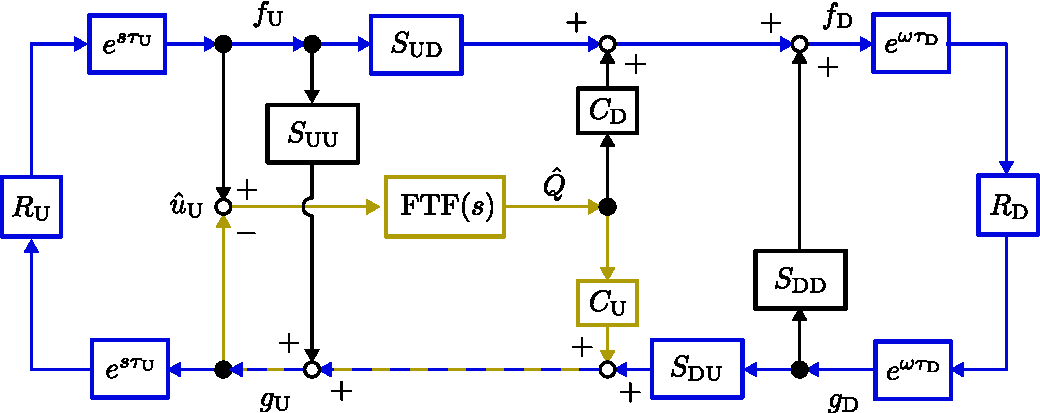
\includegraphics[scale=0.65]{assets/imgs/ITA-mech.pdf}
\caption{INTRINSIC THERMOACOUSTIC FEEDBACK LOOP}
\label{fig:ita-loop}
\end{figure}

% Doesn't need to be too elaborate!

% But there are not just acoustic modes, the full set of thermoacoustic instability modes includes ITA too [cite?]
% explain feedback loop
% phasors are cool
% some other stuff i read about
% cite the good reviews!

\cite{emmert2015IntrinsicThermoacousticInstability}
\cite{silva2023IntrinsicThermoacousticInstabilities}
\cite{hoeijmakers2014IntrinsicInstabilityFlame}
\cite{hoeijmakers2016FlameDominatedThermoacoustic}
\cite{orchini2025TrackingAcousticIntrinsic}
\cite{chen2024BiglobalLinearStability}
% Polifke?






\section{Techniques for Computational Fluid Dynamics (CFD)}

% Mention AVBP and CERFACS?

\cite{, domingo2023RecentDevelopmentsDNS, chen2011PetascaleDirectNumerical, yang2015LargeEddySimulationPresent, veynante2002TurbulentCombustionModeling, moin1998DirectNumericalSimulation, tennekes1972FirstCourseTurbulence}

The most brute force way to simulate a fluid system would be one where you try to accurately simulate every detail involved in the fluid. This idea was first studied by Orszag \cite{orszag1970AnalyticalTheoriesTurbulence}, where he defines \emph{direct numerical simulations} (DNS) as a numerical simulation with enough grid points to full resolve the smallest physical phenomena in the system. Originally, Orszag studied this in the context of turbulent flows. In turbulent flows, we have vortices not only on the order of the typical flow length scale $l_T$, called the integral length scale, but also of sizes all the way down to the smallest turbulence scale known as the kolmogorov length scale $l_K$ [CITE], where the rate at which viscous dissipation effects dampen vortices far exceeds the inertial forces of the vortex. In DNS of turbulent combustion, the smallest scale vortices must be resolved in addition to the smallest chemical length scales. In this context, the relevant time scales are chemical $τ_C = l_{\rm{th}} / S_L$, integral $τ_T = l_T / u'$ and Kolmogorov $τ_K = l_K / u'$ given an RMS velocity scale $u'$. Hence, the number of degrees of freedom required to resolve a three-dimensional box of size $L$ is:
\begin{equation}
N_{\rm{tot}} = \left( \frac{L}{2 l_T} \right)^3 \Da \: \Ka \: \rm{Re}_T^{7 / 4}
\end{equation}
where we define the turbulent Reynolds number by $\rm{Re}_T \equiv ( l_T / l_K )^{4 / 3}$, Damköhler number by $\Da \equiv τ_T / τ_C$ and Karlovitz number by $\Ka \equiv τ_C / τ_K$.


For most turbulence intensities and combustion reactions, this means having a discretisation length scale on the order of 10 - 100 $μ$m.

% The size of this kolmogorov length scale is determined by the turbulent reynolds number and the integral scale with the relationship

% A consequence of this is the extraordinary computational cost to accurately simulate a large domain. To fully resolve DNS of turbulent combustion, for example, the small chemical length scale must be resolved in addition to the smallest scale vortices. 

% An alternative method that is widely used is LES and involves using models to estimate the transfer of energy at the smallest scale rather than fully simulating them [cite les review: Yang 2015]
% DNS for turbulent combustion are reviewed in \textbf{Domingo and Vervisch 2023} (with connection to LES) and \textbf{Chen 2011}.

% For small-scale, low-speed methane-air and hydrogen-air combustion, the flows we look at have similar properties to air, so are not very viscous meaning the smallest scale vortices in a fully developed turbulent may be ~...?
% But the turbulence usually isn't our biggest worry, since we also have the thin region that the reaction is taking place to resolve, usually only 300 {\textmu}m which is resolved with ~15 nodes in a high order code
% Regardless, when performing DNS careful consideration must be made to use ample sample points

% ?? DNS with simple transport / chemical schemes?

\subsection{Mesh-free Methods}

\cite{monaghan1992SmoothedParticleHydrodynamics, vacondio2021GrandChallengesSmoothed}





\subsection{High-Order Discretisation}




\subsection{Navier-Stokes Characteristic Boundary Conditions}

\cite{thompson1987TimeDependentBoundary, thompson1990TimeDependentBoundaryConditions, poinsot1992BoundaryConditionsDirect, poinsot2005TheoreticalNumericalCombustion, sutherland2003ImprovedBoundaryConditions}

% [Thompson 1987, 1990, Poinsot and Lele 1992, Sutherland and Kennedy 2003, Poinsot and Veynante 2005]


% Many types of boundary conditions may be chosen for combustion schemes:
%% Periodic are very simple to enforce numerically so require no elaboration
%% No-slip or slip wall conditions
%% isothermal or adiabatic walls
%% acoustically reflecting or non-reflecting walls or inflow / outflow
%% In the case of inflow / outflow many more cases

% In most of these cases, we can use the formalism called characteristic boundary conditions (characteristic BCs)




% The simplest boundary conditions, i.e. those with constant (Dirichlet) boundary values (p=const), usually reflect acoustic waves back toward the interior of the domain. For most situations we want to simulate, this doesn't represent the physical situation, where we would rather pretend the medium continues outside of the computational domain. This motivates a need for boundary conditions which do not reflect acoustic waves - non-reflecting boundary conditions. The formalisms are based of characteristic waves entering / leaving the domain

% Fixed velocity inlets give full reflections, so cannot be used in a non-reflecting case.

% Immersed boundary methods are also an option and open up possibilities for boundaries not restricted specific node placement, especially for moving boundaries. But as detailed in King 2022, these a largely restricted to lower order accuracy at these boundaries (cite, and for what reason?).



\subsection{Delayed-Time Domain Impedance Boundary Conditions}


% Describe TDIBC briefly before going into time delay model!


\begin{figure}[t]
\centering
\includegraphics[scale=0.65]{example-image-a}
\caption{D-TDIBC}
\label{fig:D-TDIBC}
\end{figure}

Although many variations on TDIBC exist, the \emph{Delayed-Time Domain Impedance Boundary Conditions} (D-TDIBC) of \cite{douasbin2018DelayedtimeDomainImpedance} are particularly relevant for the simulation of thermoacoustic instabilities. By modelling the effect of an acoustic time delay, $τ$, a part of the computational domain -- say, an exhaust pipe -- may be truncated in place of a numerical boundary. Then, the response of this new boundary to incoming acoustics should be a sinusoidal Moiré pattern in the frequency domain. The proposition of \cite{douasbin2018DelayedtimeDomainImpedance} is that this pattern may be modelled via a meromorphic function of $2n$ simple poles. The location of these poles and their residues are then found in a preprocessing step as the values which minimise the least-squares fit with the desired response curve. Each time step then, the resulting constants are used to evaluate the change in acoustic variable at the boundary in such a way that no memory of previous time steps are required. 

After validating the model by testing its response to a Gaussian pressure bump, the model is compared against DNS of methane-air combustion in a 2D flame holder, where the upstream end is closed and the downstream end is open. Comparing this to DNS where the last 25 cm at the downstream end has been truncated to use D-TDIBC, they find that the time delay model accurately recovers the one-, three- and five-quarter eigenmode shapes, with small quantitative errors in their sound spectra. Considering the $\sim 13\%$ reduction in degrees of freedom in the computational domain resulting from the truncation, this can be seen as an impressive recovery of the problem's physics by using what is essentially a one-dimensional low-order model in the truncated region for the acoustics. Since the model constants are calculated as a preprocessing step, the envelope of the acoustic response in the frequency domain may essentially be changed arbitrarily, presenting a benefit in case different pass bands are desired.

Besides the inevitable drawbacks stemming from: the low-order model's inaccuracy and the requirement of a strongly one-dimensional flow at the boundary to match this model, other drawbacks remain prevalent. For one, no method to visualise acoustics residing in the fictitious, truncated domain is provided, potentially leading to a \emph{black-box} of energy where acoustics are essentially stored, but not known. For another, the preprocessing steps are required for each value of $τ$ used. So, if the time delay were to change dynamically during the simulation (e.g. due to an expanding computational domain to ensure the flame remains within), this preprocessing may happen each step, becoming computationally costly.





